\section{CityScope Playground}\label{sec:cityscope_playground}

{
    \subsection{Introduction}
    {
        In complex decision-making processes, stakeholders from varying backgrounds and expertise are involved. The existing frameworks for city-planning are often designed around certain professional audiences (e.g., planners and architects) and are usually less accessible to a wider scope of users \cite{ben-joseph2001}. A collaborative interactive system could facilitate stakeholder dialogues and interactions, and consequently help them make more informative decisions in shorter time.
        \newline
        This work examines user engagement and decision-making in the context of urban-regulations and zoning. The objectives of this study are twofold: (i) to examine user interactions with tangible user interfaces for urban-planning, and (ii) to investigate stakeholders' engagement and decision-making using these tools.
        This observational study was conducted with a representative sample of users from different backgrounds. These were invited to examine the usability of a CityScope variant developed in 2015, called `Playground'. A comparative analysis of different approaches examined the users' interaction and decision-making using CityScope, in comparison to traditional planning aids. The sessions involved decision-making scenarios using paper-based planning documents, alongside an interactive tangible models of the design area. A coding scheme was developed for analyzing video observations, to examine the wide spectrum of actions, verbal cues, and non-verbal gestures, and quantify the occurrences of these interactions during the experiment.
    }

    \begin{figure}[!htb]
        \begin{center}
            \includegraphics[width=1\textwidth]{chapters/transformation/playground/figures/playground.jpeg}
        \end{center}
        \caption{Impact of zoning-codes and building regulations on urban form. (top) Hugh Ferriss's drawings of NYC 1916 Zoning Ordinance (1922), the first in the United States to regulate building use, floor area, and height of new buildings. (bottom) The effect of zoning on built form and function in Midtown Manhattan.}
        \label{fig:pg_nyc}
    \end{figure}

    \subsubsection{Evaluating UHCI}
    {
        Technologies to support stakeholders in the decision-making process have evolved over the past few decades (see Chapter \eqref{chapter:introduction}). Intuitive tools can create collaborative interaction spaces, where users efficiently work with each other and see the result of their interaction immediately \cite{ishii2002augmented}. Nevertheless, studying the usability and efficiency of such systems is relatively unexplored \cite{Innes2016}.
        \newline
        Several observational studies have been conducted on TUI. Brereton and McGarry \cite{brereton2000observational} tested the usability of tangible objects, and how TUI encourages engineers' design thinking and communication. Fjeld and Sissel \cite{fjeld2002alternative} tested the usability of TUI compared to alternative traditional 3D and 2D single user tools, by examining the learning effect and the overall user experience. These studies showed that 3D tools outperformed in terms of user satisfaction. Falcao and Price \cite{price2009effect} focused on investigating collaborative activities in a tangible table-top environment, to support how shared interfaces affect the way collaborative activities are structured, and examines the kinds of interactions that are productive for learning. Ben-Joseph examined the Luminous Planning Table (LPT) \cite{ben-joseph2001}, in order to further develop its functionality based on feedback from end-users through implementation of an actual parcel slated for development.
        \newline
        This observational study examines the usability of CityScope in a simulated urban-planning process, and investigates its effect on stakeholders' engagement and decision-making. The study aimed to improve the understanding of how a mixture of TUI and virtual environments might encourage collaboration and communication among stakeholders, and lead to better decision making.
    }

    \subsubsection{Kendall Square: Site and Context}
    {
        The study examined user engagement in the context of an early stage city-planning. At this stage, zoning-laws and building-regulations are leading many of the design decisions, and are responsible to the creation of `zoning envelopes': legal frameworks to which the development of new buildings and landscapes is bounded \cite{n15, Ben-Joseph2004}. The preliminary stage of most planning processes is a comprehensive understanding of the spatial and regulatory context. Figure \eqref{fig:pg_nyc} shows the impact of zoning on urban form in NYC.

        \begin{figure}[!htb]
            \begin{center}
                \includegraphics[width=.75\textwidth]{chapters/transformation/playground/figures/playground0.png}
            \end{center}
            \caption{Kendall Square and MIT east-campus. CityScope Playground was used in this observational study to investigate the usability of the TRP system in the context of the MIT east-campus redevelopment project (photo: MIT).}
            \label{fig:pg_kendall_site}
        \end{figure}

        \textbf{Site:} Kendall Sq. in Cambridge, MA, was chosen for this case study. The unique features of this area\footnote{Kendall Sq. is sitting on the verge of MIT, has adjacency to low-density, low-income neighborhoods, close to Boston CBD, and surrounded by unique geographical features.} creates additional interest for the study of regulatory frameworks and their impact on new development (see Figure \eqref{fig:pg_kendall_site} for the redevelopment site used in this study). During the past few decades, the post-industrial area of Kendall Sq. reemerged as a technological hub. Several planning effort were initiated to increase capacity for MIT eastern campus and the adjacent area, aiming to update current height limits, AOR, GFA and other regulations\footnote{See Appendix \eqref{appendix:playground} for the history and a list of redevelopment efforts in the Kendall area.}.
        \newline
        \textbf{Zoning and Regulation:} Kendall Square was intensively planned over the years. Due to its history, location, and unique geography, the site intersects multiple zoning areas. From the south-east, the MIT main campus has mostly low-rise buildings and continuous facades, stretching along Main street and Memorial drive; From the north, a mixture of high-rise office towers, medium-rise condominiums, and low post-industrial structures; In the north-west, low-rise and residential buildings. Over the years, these typologies created a massive trail of zoning and regulations, which can be challenging to distill even by professionals\footnote{An example of this ambiguity could be found in the K2C2 study (Kendall and Central squares), commissioned by the city in early 2011 in response to interest in increased development capacity. Although the study guidelines represent thorough research done in order to improve redevelopment efforts, the legal status of these recommendations is unclear: \begin{quotation} ``The Kendall Square Design Guidelines are created... to \textbf{inform} property owners, business owners, developers, and the general public about the desired form and character of development in Kendall Square...However, the guidelines are not intended to impose a strict limitation on the building form and style. Other creative design solutions, or measures, not noted here may also be utilized to achieve the same goals at the discretion of the Planning Board..." \end{quotation}}.
    }

    \subsection{Tangible Regulation Platform}

    {
        This user study compares two different urban-planning methodologies: (i) Classic, `pen-and-paper' decision-making, and (ii) A digital-physical decision support system. The comparison is meant to enhance the differences between an evidence-based urban-planning session, and a traditional one.
        The Tangible Regulation Platform (TRP) is a CityScope variant designed to evaluate urban-design proposals in the context of zoning-laws and regulations. Users input is examined in real-time, to reflect their impact on the built environment, and to offer an early assessment of the buildable zoning envelopes. For example, a community undergoing a redevelopment initiative, could benefit from the TRP to preform zoning simulation, sometimes years before actual development is taking place. Figure \eqref{fig:pg_trp} shows the TRP setup and usage.
        \newline
        The TRP is composed out of three components: (i) A physical 3D urban model, (ii) a computational unit, and (iii) a feedback module. The computational unit is responsible for evaluating the city regulations and guidelines in response to users input. These algorithms compile zoning, code, and regulations into virtual envelopes, mimicking to the way a municipal board would evaluate a development proposal. Figure \eqref{fig:pg_module} describe the zoning simulation module.
    }

    \begin{figure}[!htb]
        \begin{center}
            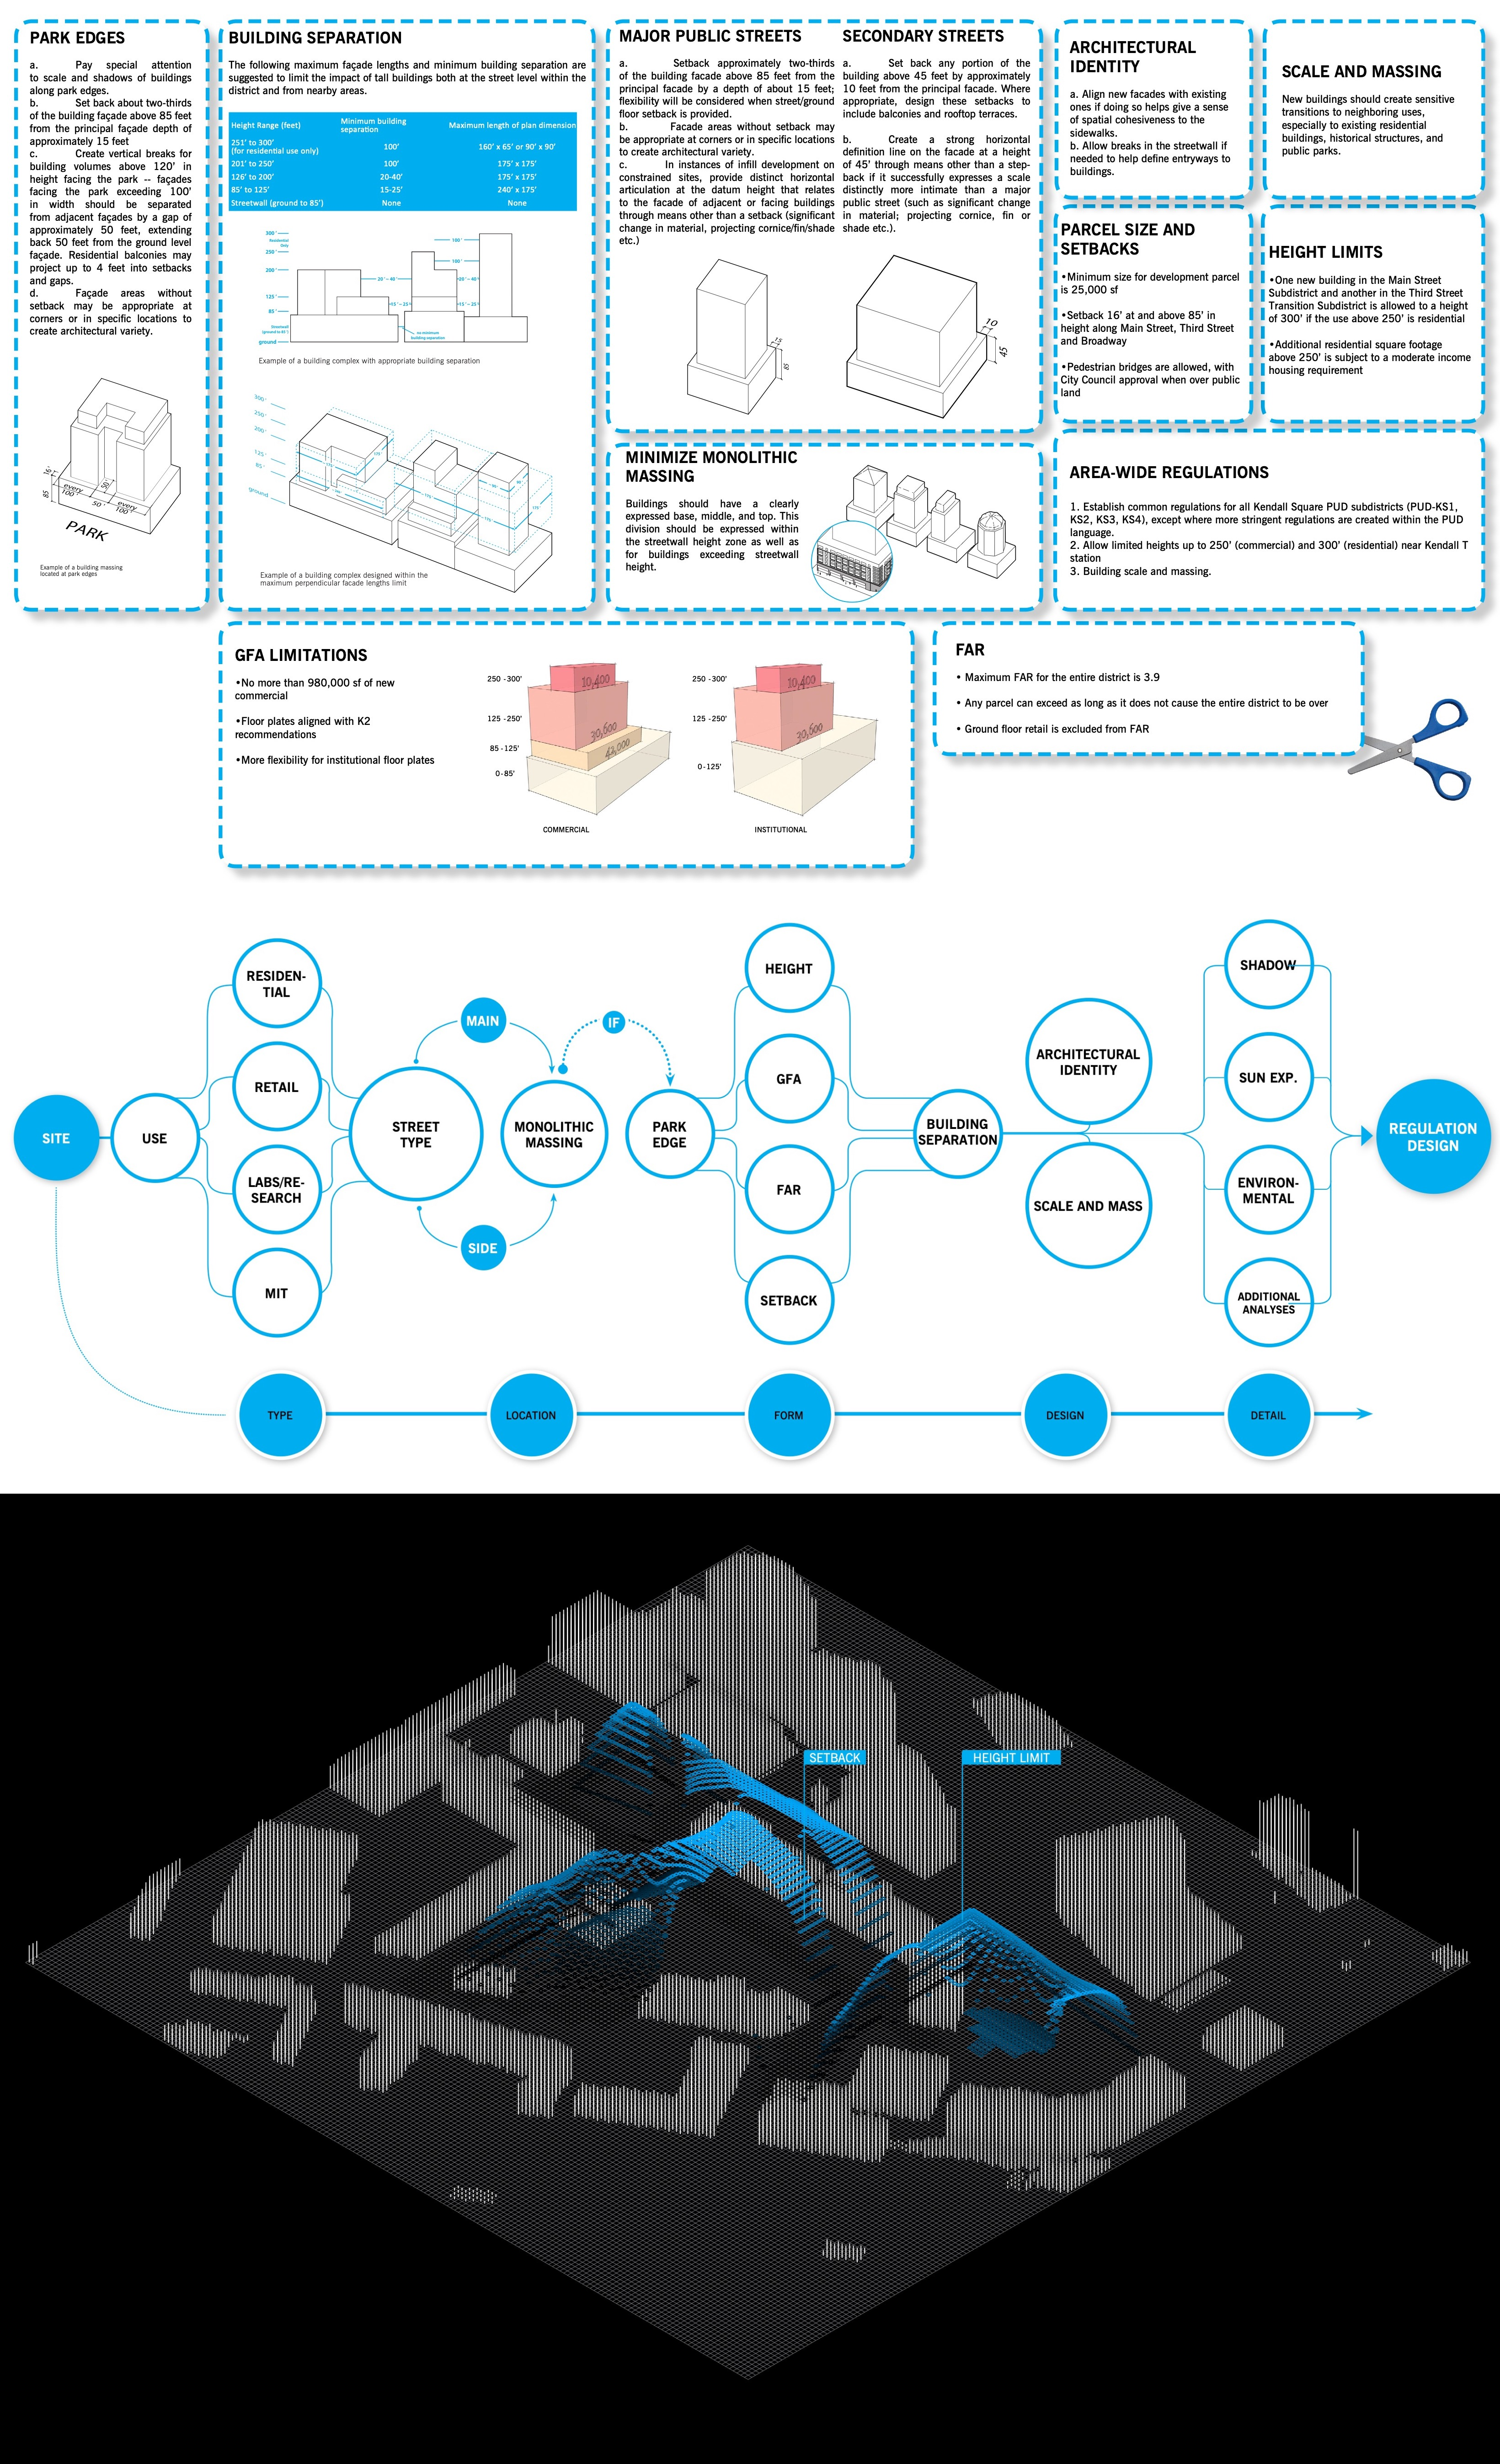
\includegraphics[width=0.65\textwidth]{chapters/transformation/playground/figures/playground2.png}
        \end{center}
        \caption{The `zoning simulator'. (from the top) A subset of the zoning amendments proposed for this site was used for modelling the TRP. The zoning codes and building regulations were converted to logical methods (center), and then linked to other methods to evaluate each design proposal. Finally, the results of the simulation was visualized (bottom).}
        \label{fig:pg_module}
    \end{figure}

    \subsubsection{The TRP TUI}
    {
        The TRP includes (i) an array of tagged 3D objects, serving as massing elements of zoning envelopes, (ii) a table that constrains the placement of 3D objects into an urban context, (iii) sensors for scanning the scene, computers, display screens, and projectors for projecting light patterns onto the table. The TRP tabletop is composed of a physical grid of 192x192 LEGO bricks; The grid represents two conditions: (i) `fixed': the non-modifiable parts of the city, and (ii) the `playground': the interactive part of the TRP. A user places physical objects into indentations which form a grid on the table; The objects are then scanned and digitally reconstructed (see Section \eqref{subsec:csarch-cityscopy} for technical description of scanning and parsing the table's state).
        \newline
        Similar to digital monitors, the `resolution' of the table - the density of pixels for a given area - is a key parameter which dictates interaction, simulation, and feedback. Unlike meticulously crafted urban maquettes, the `roughness' of the pixelated CityScope model is intentionally shifting the focus from design details to the overall scheme, massing, and relationships between functions.
        When designing the platform, the smallest tile should represent the smallest unit of interaction and analysis. This decision stems not only from the physical aspects of the urban context, but also from the smallest analytical unit. In the case of the TRP platform, this measurement was based on the smallest unit being used in the site's zoning documents, equal to ~8ft\footnote{The smallest unit was found in an 8ft setback rule, imposed on low-rise building parcels of side streets. This rule was set as the smallest sampling unit for the entire urban model and consequently - for the buildings' height and appearance.}.
    }

    \subsubsection{Types System}\label{subsec:playground_types_system}

    {
        A set of rectangular blocks was defined as the `Bank'. The blocks, different in height but equal in their footprint, are a collection of 16 unique `zoning elements'. Each element retains two parameters: land-use and height, and each block can hold more than one land-use; For example, one block with 22 floors may include 3 floors of retail space in the street level, and 19 floors of residential or office space above. Here, a single block cannot represent a building; In order to construct a viable building envelope, each of the given blocks must be attached to others. The assemblage of these blocks creates zoning envelopes that are diverse in size and program, thus creating a complex zoning environment\footnote{CityScope Playground used an early data scheme to represent the table's state and interaction. For the CityScope Schema, see Section \eqref{sec:cityscope_architecture}.}.
    }

    \subsubsection{Feedback Module}

    {
        \textbf{Scanning And Evaluation:} When users change the configuration of the 3D objects array, the digital reconstruction of the CityScope grid is analysed in relations to the zoning and regulation. The output of this analysis is plotted as a visualization to both the tabletop and a set of vertical monitors. The users then react to the feedback in their next interaction with the TRP.
        \newline
        \textbf{Feedback Devices:} The TUI setup consists of two output devices: Array of 4 projectors, mounted to the room's ceiling above the table corners; The projectors are synced to the 3D models shape using projection mapping. The projectors display data visualization corresponding to users` interaction, so that changes made to the physical model will be visually echoed.
        The second part of the feedback module is a TV dashboard, synced with the projected visualization. Information displayed on the screen is (i) GFA calculation for new additions and for existing urban context; (ii) Percentage of buildings using or exceeding existing FAR; (iii) Open space and built-area ratios; (iv) Occupancy and sub-sectioning of each land-use.

    }

    \subsection{Observational Study}

    {
        The observational study was conducted with a representative sample of users from different backgrounds. The users were randomly invited to examine the usability of the TRP, and to express their opinion on ways to improve planning processes through such platforms. The sessions involved decision-making and design scenarios using artifacts such as paper-based sketching, note-taking, as well as verbal discussions. All sessions were recorded and analyzed; A coding scheme was developed for analyzing the video observations, in order to examine the wide spectrum of actions, verbal cues, and non-verbal gestures, as well as quantify the occurrences of these interactions during the experiment.


        \begin{figure}[!htb]
            \begin{center}
                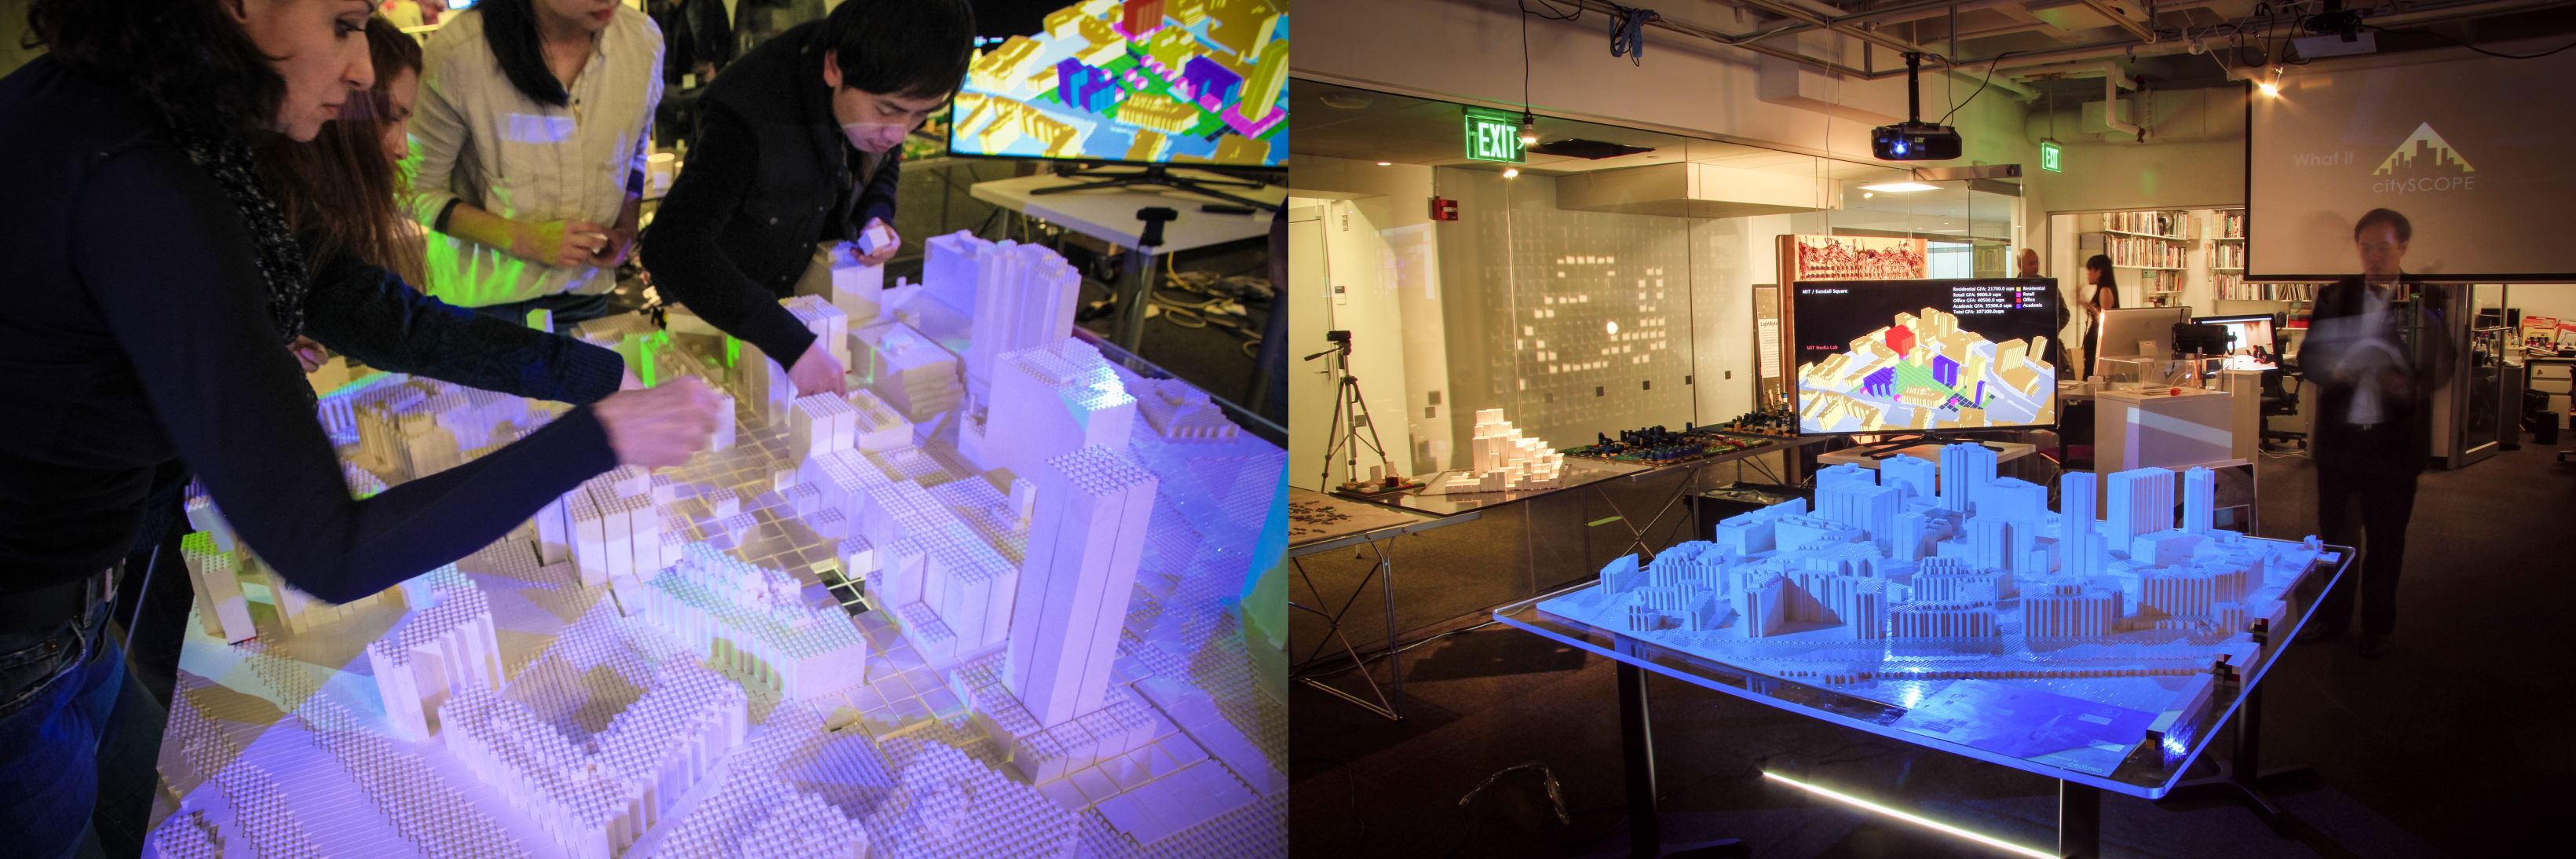
\includegraphics[width=1\textwidth]{chapters/transformation/playground/figures/playground1.png}
            \end{center}
            \caption{CityScope Playground and the TRP. (right) Overview of the complete system, including the TUI, feedback module, and the `Bank'. (left) The TUI in use during the experiment. Users can collaboratively interact, discuss, and improve their design based on feedback from their peers and the system's responses.}
            \label{fig:pg_trp}
        \end{figure}

        Fifteen participants from the MIT community, including students, staff, and affiliates were invited through an open, unrestricted online form, email lists, and in-campus publications. Upon arrival, the participants were divided into two groups: \textbf{Community Meeting session:} This group held a paper-based discussion, and later moved to the \textbf{TRP session:} In which participants were invited to use the interactive tangible model.  Recording was done using Morae \cite{techsmit94:online}, a usability testing tool to record and analyze multiparty sessions.


        \subsubsection{Procedure}
        {
            In each of the sessions, participants were asked to respond to real-life planning and design challenges in the Kendall Sq. area. At the beginning of the day, the groups were informed about past and existing master-plans and zoning restrictions imposed on the site. They were then asked to rebuild and plan the Kendall Sq. area, taking into account zoning restrictions by adding residential, commercial buildings, parking lots, parks and public amenities. In the TRP session, participants were asked to do the same, while interacting with the CityScope platform. The TRP real-time feedback notified the user whenever a violation of the zoning restrictions occurs in their design, through visualization, text, and symbols.
        }




        \begin{figure}[!htb]
            \begin{center}
                \includegraphics[width=1\textwidth]{chapters/transformation/playground/figures/playground3.png}
            \end{center}
            \caption{User interaction and TRP feedback. As users interact with the TRP, the system evaluates the design based on the zoning simulator module. As users progress with their spatial design, the system highlights violations of the zoning-laws and building-codes, allowing the user to align their design or otherwise challenge the zoning rules.}
            \label{fig:pg_interaction}
        \end{figure}


        \subsubsection{Analysis}

        {
            The video recordings of the sessions were analyzed using a coding scheme. The different types of coding schemes, actions, verbal and non-verbal behaviors are described in Table \eqref{tab:coding_scheme}; Results of the analysis are presented in the Appendix Table \eqref{appendix:coding_scheme_results}.

            \begin{table}
                \begin{center}
                    \caption{Coding Schemes}
                    \label{tab:coding_scheme}
                    \begin{tabular}{l|ll|ll}
                        Code & Description           & Code & Description                              & \\

                        \noalign{\hrule height 0.5pt}

                        EXP  & Explore Function/Tool & EXT  & Excitement                               & \\
                        PUZ  & Puzzled               & SUR  & Surprised                                & \\
                        CLA  & Clarification of Idea & ACT  & Wrong Action                             & \\
                        IDE  & Introduction of Idea  & FRT  & Frustration                              & \\
                        ACC  & Acceptance of Idea    & DIS  & Discontinuous Action                     & \\
                        EVA  & Evaluation of Idea    & REC  & Recognition of Error or Misunderstanding & \\
                        REF  & Refinement of Idea    & DBT  & Doubt                                    & \\
                        HAN  & Hand over             & COR  & Corrective Action                        & \\
                        HES  & Hesitation            & FLO  & Floor-Holding                            & \\
                        DIF  & Execution Difficulty  & TAS  & Give Task to Another User                & \\
                        EXE  & Execution Problem     & SCH  & Search for Non-Existing Function         &
                    \end{tabular}
                \end{center}
            \end{table}
        }
    }

    \subsection{Results and Findings}

    {
        The video recordings of each session was analyzed using the predetermined coding scheme. This scheme included several types of actions, verbal and non-verbal behaviors, and physical gestures. The coding scheme helped recognizing behavioral patterns in the different sessions. For example, it was apparent that most participants spend the first part of their session exploring the TRP and searching its basic functionality, as noted by the multiple occurrences of $EXP$ and $SCH$ codes. Therefore, it can be assumed that a demonstration of the system would make users more comfortable interacting with it. The occurrences of code $IDE$ indicates that dealing with physical objects made participants more active and engaged in the planning and decision-making process. The $ACC$ code reflects that due to the feedback visualization, participants shared a common understanding of the proposed plan. As indicated in the multiple occurrences of $CLA$ and $EVA$ codes, the attention to zoning violation was greater while using the TRP due to real-time feedback. Unlike traditional sketching methods, where participants might not consider zoning, the TUI assisted participants in identifying violations of the zoning restrictions.
        \newline
        In terms of TUI design, the systems was found to cause some frustration and confusion (which is noted in codes $FRT$ and $PUZ$) when participants could not differentiate between removable and fixed physical objects, and when they indicated difficulties in identifying an object. These observations revealed opportunities for improving the user experience of the TUI system\footnote{For full breakdown of the coding scheme results, see Table \eqref{tab:coding_scheme} in the Appendix.}.
    }


    \subsection{Discussion}
    {
        In order to design successful UHCI systems that supports collaboration and facilitate decision-making between stakeholders, it is essential to test their usability in real-world scenarios.
        This study analyzes the usability of a Tangible Regulation Platform (TRP) system, by applying a coding scheme on recorded observations of users' experience, and decoding them to asses usability, and interaction. These findings suggest that UHCI are superior to traditional urban-planning methods in terms of rapid prototyping, collaboration, and decision-making processes.

        \subsubsection{Strengths}
        {
            The TRP platform had several key technological and operational advancements over prior art: This platform was the first large scale CityScope that incorporated real-time interaction, feedback, and participation, all in one system. Despite analyzing unconventional metric such as zoning laws, the TRP feedback was proven to be effective in user experiments.
        }

        \subsubsection{Challenges}

        {
            Evaluating the platform within the confines of the Media Lab building had several limitations. First, intervention in an existing urban-design proposal should involve stakeholders or communities that have direct relations to the site in question. Amongst the visitors, only few were local residents who generally shared a wide and inconsistent degree of acquaintance with the site.
            Second, the TRP zoning analysis could not be evaluated against the actual process of zoning evaluation by the city. In later CityScope projects, evaluations and analysis would be comparative to the actual evaluation process (for example, see the Grasbrook project \eqref{sec:grasbrook}).
        }

        \subsubsection{Opportunities}
        {
            A key finding emerging from both formal and informal feedback, was that participants desired to not only use the TRP to evaluate zoning, regulations, and building-code, but also to use it for other urban performance metrics. As such, municipalities or public officials may test walkability and transportation concerns; The quality of open landscapes, public amenities and civic safety can be tested in existing or amended regulations; Potential ROI, revenues, or market-appeal of properties can be assessed prior to regulatory amendments.
        }
        \newline
        These findings paved the way to a more holistic approach in the design, development, and deployment of future CityScope platforms. The rest of this Chapter details a unified CityScope platform which is set to answer multiple spatial questions, and to be used by multiple stakeholders, settings, and stages of the planning process (see \eqref{sec:cityscope_architecture}, \eqref{sec:grasbrook}).

    }
}